\documentclass[rapport.tex]{subfiles}
\begin{document}
    \chapter{Projets}
        \section{Jobigo}\label{subsec:jobigo}
        \begin{wrapfigure}{l}{0.25\textwidth}
            \centering
            
\includegraphics[width=0.25\textwidth]{jobigo_logo}
        \end{wrapfigure}
        Au tout début de mon stage, j'ai été assigné à un projet déjà en cours~:~\emph{Jobigo}.\
        l'objectif de
        ce projet était de permettre à chacun de trouver du travail plus facilement
        en mettant en relation chercheur d'emploi, et employeurs.
        Le projet était quasiment terminé au moment où je suis arrivé, il s'agissait simplement d'ajouter
        les derniers détails pour que l'\gls{api} puisse interagir avec l'application mobile
        de façon optimale.

        Le processus de création d'une \gls{api} implique de pouvoir lister toutes les actions 
        qu'il sera possible de réaliser sur l'application, comme par exemple, la connexion d'un utilisateur, 
        ou la création d'une offre d'emploi dans le cadre de jobigo.


        \subsection{Architecture utilisée}
        Le projet a été construit en utilisant le patterm \gls{mvc}
        afin d'avoir une architecture evolutive, et surtout maintenable. Dans
        le cadre de jobigo, cette architecture peut-être résumé comme dans la
        figure \ref{fig:jobigo}.
        En réalité, toutes les actions que l'on peut faire sur un site web se
        font au travers d'un controller, et lorsque l'on explore un site web,
        il y a un jeu de question/réponse entre l'ordinateur et le serveur qui
        héberge le site. Dans le cadre de Jobigo, il ne s'agit pas d'un
        ordinateur, mais d'une application qui envoie des requêtes au serveur.

        Le controleur que l'on peut voir sur la figure \ref{fig:jobigo} est
        donc le point d'entrée de \gls{api} pour n'importe quel utilisateur.
        C'est lui qui sera responsable de~: 
        \begin{itemize}
            \item Vérifier que l'utilisateur est authentifié : il s'est connecté au travers de l'application
            \item s'assurer que l'utilisateur a le droit d'accéder aux informations qu'il demande
            \item D'aller chercher les informations demandée
            \item Mettre en forme les données, dans le cadre de jobigo, les données sont formatées en \gls{json}
        \end{itemize}

        \begin{figure}
            \centering
            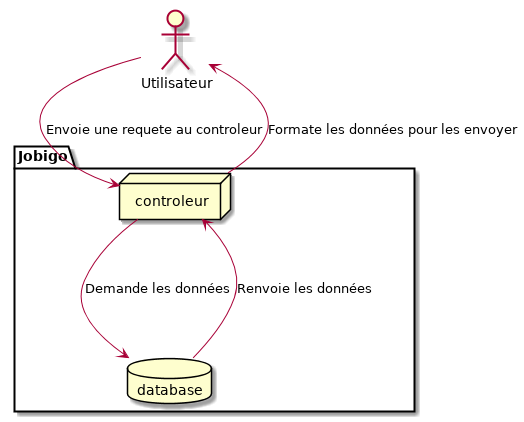
\includegraphics[scale=0.5]{jobigo}
            \caption{Plan de l'architecture}
            \label{fig:jobigo}
        \end{figure}

        Avec cette manière de procéder, il est très facile d'ajouter des actions
        à l'\gls{api}.

        Il existe des conventions pour concevoir une API, comme la convention \gls{rest} qui a été utilisée
        sur ce projet, mais également sur mynabes\footnote{cf page \pageref{subsec:mynabes}}. Elle permet
        notamment de centrer la conception de l'\gls{api} sur les resources qui vont être utilisées.
        Dans le cadre de Jobigo, une resource peut être une offre d'emploi.

        \gls{rest} permet d'établir les différent chemin disponible dans la table \ref{table:rest}, et permet très rapidement
        de définir toutes les \glspl{url}, mais aussi de comprendre à quoi servent chacune d'entre-elles dans le projet

        \begin{table}
        \begin{tabular}{|r|l|r|}
            \hline
            Méthode HTTP & url & Description\\
            \hline
            \textit{GET} & /job/\{id\} & Obtenir le post correspondant à l'id\\ 
            \textit{POST} & /job/ & Créer un job\\
            \textit{PUT} & /job/\{id\} & Mettre à jour un job\\
            \textit{DELETE} & /job/\{id\} & Supprimer un job\\
            \textit{POST} & /job/\{id\}/apply & Postuler à une offre\\
            \hline
        \end{tabular}
            \caption{Application de la convention REST}\label{table:rest}
        \end{table}

        \subsection{Technologies utilisées}

        \begin{center}
        \begin{minipage}{2.5cm}
            
\includegraphics[scale=0.2]{docker}
        \end{minipage}
        \begin{minipage}{2.5cm}
            
\includegraphics[scale=0.1]{gitlab}
        \end{minipage}
        \begin{minipage}{3cm}
            
\includegraphics[scale=0.1]{jenkins}
        \end{minipage}
        \begin{minipage}{2.5cm}
            
\includegraphics[scale=0.2]{crashlytics}
        \end{minipage}
        \begin{minipage}{2.5cm}
            
\includegraphics[scale=0.15]{apiplat}
        \end{minipage}
    \end{center}

        Implémenter l'architecture définie pour Jobigo requiert de faire des choix technologiques.
        L'\gls{api} a été construite en php avec api platforme\cite{apip}.
        Pour s'assurer que l'environement de l'\gls{api} est le même chez tous les developpeurs, et sur le
        \gls{prod}, l'\gls{api} a été encapsulée dans un \gls{cont} grâce à \textit{Docker}. Docker propose
        tout un écosystème de container, et chacun peut écrire ou modifier le code d'un container afin
        de l'adapter à ces besoins et éventuellement de partager le nouveau container ainsi créer.

        L'équipe chargée de travailler côté serveur était composée de trois personnes, moi y compris.
        Cela introduit un problème : comment collaborer sur une meme base de code ? En vérité personne ne se pose
        la question, la réponse est déjà toute trouvée~:~il suffit d'utiliser \emph{git} et d'heberger le code
        sur l'un des sites qui en propose le service. Git permet à plusieurs développeur de disposer d'une copie du code
        et de gérer la mise en commun. 

        Pour finir, le projet a été développer en mettant en place une stratégie d'intégration continue.
        Ainsi, toutes modifications validées par le chef de projet est disponible automatiquement pour le client.
        Ce dernier dispose ainsi systématiquement d'un site utilisable et il peut lui même constater l'avancement du projet.
        L'\gls{api} en elle même était déployée grâce à jenkins, l'application quant à elle était déployée grâce à crashlytics.
        Crashlytics permet au client d'être notifié de chaque nouvelle version utilisable de l'application, sans passer par un store officiel.
        Il a ainsi la possibilité d'installer l'application, la tester, et faire ses retours.

        \subsection{Les notifications push}
        Avec la démocratisation des smartphones, il y a eu une explosion de l'utilisation des notifications. C'est donc tout naturellement
        qu'il a fallu développer un mécanisme pour notifier les utilisateurs
        des événement relatif à jobigo.
        Les notifications push ne sont pas envoyée directement depuis le
        serveur, il faut faire appel à l'un des services proposé par Google
        (FCM, pour les appareils Android ou iOS) ou Apple (APNS, seulement pour
        iOS). Dans le cadre de jobigo, il a été décidé d'utiliser conjointement
        FCM et APNS.
        La figure \ref{fig:notification} résume le principe de fonctionnement des notifications push.

        \begin{figure}
            \centering
            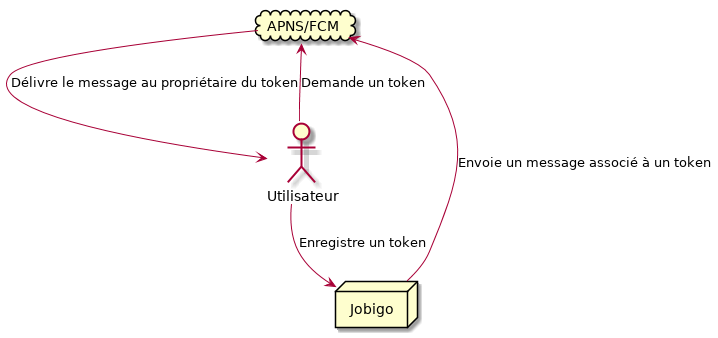
\includegraphics[scale=0.5]{notification}
            \caption{Fonctionnement des notifications push}
            \label{fig:notification}
        \end{figure}

        Un token est simplement un identifiant pour un appareil, un smartphone
        par exemple. Pourtant, Intuitivement on voudrait envoyer un message à
        une addresse qui identifie directement le smartphone d'un utilisateur,
        comme son addresse IP par exemple. Cependant procéder comme tel
        introduirait plusieurs problèmes~:
    \begin{itemize}
        \item L'IP n'est pas fixe (surtout avec un mobile) : il faudrait garder
            une trace des changements et forcer l'application à mettre à jour l'addresse IP à chaque
            changement : \textbf{c'est un traitement lourd}
        \item Si la sécurité du site est compromise, les addresses IP de tous
            les utilisateurs sont compromises : \textbf{c'est grave}
    \end{itemize}
        utiliser un token permet de déléguer toute la gestion des notifications à un service externe, qui lui s'occupera des deux problèmes
        cités précédemment.

        Cependant faire appel à un service externe ne décharge pas de toutes les responsabilités.
        Il reste malgré tous la gestion de l'enregistrement des \glspl{token} au sein de l'\gls{api}.
        Il a ainsi fallu rajouter la possibilité pour l'application de pouvoir enregistrer un \gls{token} grâce à l'\gls{api}.
        Dans le cas rare, mais possible, où un \gls{token} serait déjà utilisé, il a également fallu rajouter
        une procédure pour changer la propriété du \gls{token}. De cette manière si le \gls{token} était déjà utilisé, 
        il est réattribué à la dernière personne qui en a fait la demande.

        L'utilisateur peut en outre choisir de ne pas recevoir certains types de notifications, comme par exemple une notification de refus.
        Dans ce cas il fallait aussi prendre ce paramètre en compte au cas par cas.

        \subsection{Problèmes rencontrés}
        L'un des principales difficultés que j'ai rencontré sur ce projet était
        l'utilisation de technologies qui étaient nouvelles pour moi.
        Les deux premières semaines ont donc été assez lourdes, puisqu'il a
        fallu que j'apprenne ce qu'était par exemple un token JWT pour
        l'authentification des utilisateurs, que je comprenne comment Docker
        était utilisé pour simplifier le déploiement du projet.

        Une autre difficulté qui est apparue vers la fin du projet a été le
        traitement asynchrone des notifications. En effet, envoyer des
        notifications nécessite de se connecter à un service externe,
        d'attendre la réponse, puis renvoyer une réponse à l'utilisateur.
        Seulement l'utilisateur n'a pas d'intérêt à attendre que google
        confirme que la notification a été envoyée. Normalement ce problème ce
        règle en exécutant ce traitement en arrière plan. Seulement php ne
        permet pas de le faire de manière simple.

        Le fait également qu'il a fallu travailler avec FCM et APNS pour les
        notifications Apple et Android a été compliqué dans le sens où les deux
        services ne traitent pas exactement les notifications de la même
        manières, les données à fournir ne sont pas exactement les mêmes. Il a
        donc été nécessaire de traiter les deux cas de manière différente sans
        rendre le code illisible.

        \section{Smart ULD}
        \begin{wrapfigure}{l}{0.25\textwidth}
            \centering
            
\includegraphics[width=0.25\textwidth]{sita}
        \end{wrapfigure}
        Une fois ce projet livré, j'ai été assigné à un autre projet.
        Le client en question, SITA,  développe un projet permettant de suivre des container
        à bord des avions, et notamment suivre leur geolocalisation.
        Pour que ce flux de données soit correctement acheminé, une architecture à base de micro-services
        avait déjà été prototypée par le client. Le but pour Siclo était donc à
        partir du prototype, de 
        redévelopper un ensemble de micro-services un peu plus robustes. Un
        résumé de l'architecture est disponible figure~\ref{fig:overview}. L'objectif final de cette chaine de micro-services est de pouvoir stocker les données dans la base mongodb.
        \sub
        \subsection{Architecture utilisée}
            Le projet était déjà existant, par conséquent l'arhitecture était imposée par le client.
            Comme dit précédemment il s'agissait ici d'un ensemble de micro-services. Le principe 
            est de limiter chaque micro-service à une seule tâche. C'est une application du
            principe de responsabilité unique que l'on peut retrouver dans la convention \gls{solid}. Procéder de cette manière a plusieurs avantages~:~
            \begin{itemize}
                \item Le code en devient plus lisible, il n'y a pas un seul
                    \og gros\fg programme à lire
                \item La maintenance s'en trouve facilitée, puisque chaque
                    micro-service à un code source
                    plus petit, il est facile d'identifier un bug, puis de le résoudre
                \item il est également plus facile de remplacer les
                    micro-service en cas de besoins, 
                    voire d'en introduire des répliques dans le processus à des fins de test.
                \item Avec un ensemble de micro-services, il est également plus
                    facile d'allouer plus de ressources (mémoire/performance)
                    à un service qui en aurait besoin, et en retirer pour des
                    services qui ne consomme pas beaucoup. Ce qui est
                    totalement 
                    impossible pour un programme monolithique
            \end{itemize}
            Tous les micro-services sont liés les uns aux autres grâce à des
            queues. Une queue fonctionne sur le modèle \gls{fifo}. Cela permet de placer toutes les données dans
            des files d'attentes, et de les traiter en fonction de leur ordre
            d'arrivée. Utiliser un système de queues permet aussi, au besoin, de
            mettre plusieurs services en entrée ou sortie de
            queue afin d'améliorer les performances de toute la chaine de
            micro-service. Utiliser un système de queues permet aussi de ne pas perdre de données si l'un des micro-service
            est hors-ligne. Dans ce cas, les données restent dans la queue en attendant d'être traitée. Ce ne serait pas
            possible si tous les micro-services étaient connectés directement entre eux.
        \subsection{Technologies utilisées}
        Ces micro-services ont été écrits en NodeJS\cite{node} avec typescript.
            Typescript permet d'écrire du code en javascript en rajoutant la notion de
            typage sur l'ensemble des variables, ce qui permet d'écrire un code
            d'une part
            plus lisible, et d'autre part vérifié par un compilateur. Ce qui en
            fait un code plus sûr.

            Tous les services sont liés par des queues RabbitMQ\cite{rmq}, qui est une implémentation du protocole AMQ. 

            La base de données principale est une base de données orientée
            document, MongoDB. L'avantage de ce type de base de données est
            qu'il n'y a pas de vraies définition de données, on peut stocker
            n'importe quoi à partir du moment où le format utilisé est le
            \gls{json}. Par rapport au contexte du projet, et vu la masse de
            données à traiter, c'était le meilleur choix pour ne pas ralentir
            la chaine, Puisque la vitesse d'insertion et de lecture dans ce
            type de base de données est supérieure par rapport à une base de données
            relationnelles, comme MySQL par exemple.
            Le projet est encore en phase de test, par conséquent le modèle de
            données peut encore évoluer. Utiliser un système de base de données
            sans définition de schéma est donc plus pratique. Le schéma
            peut-être établi plus tard.

        \begin{figure}
            \centering
            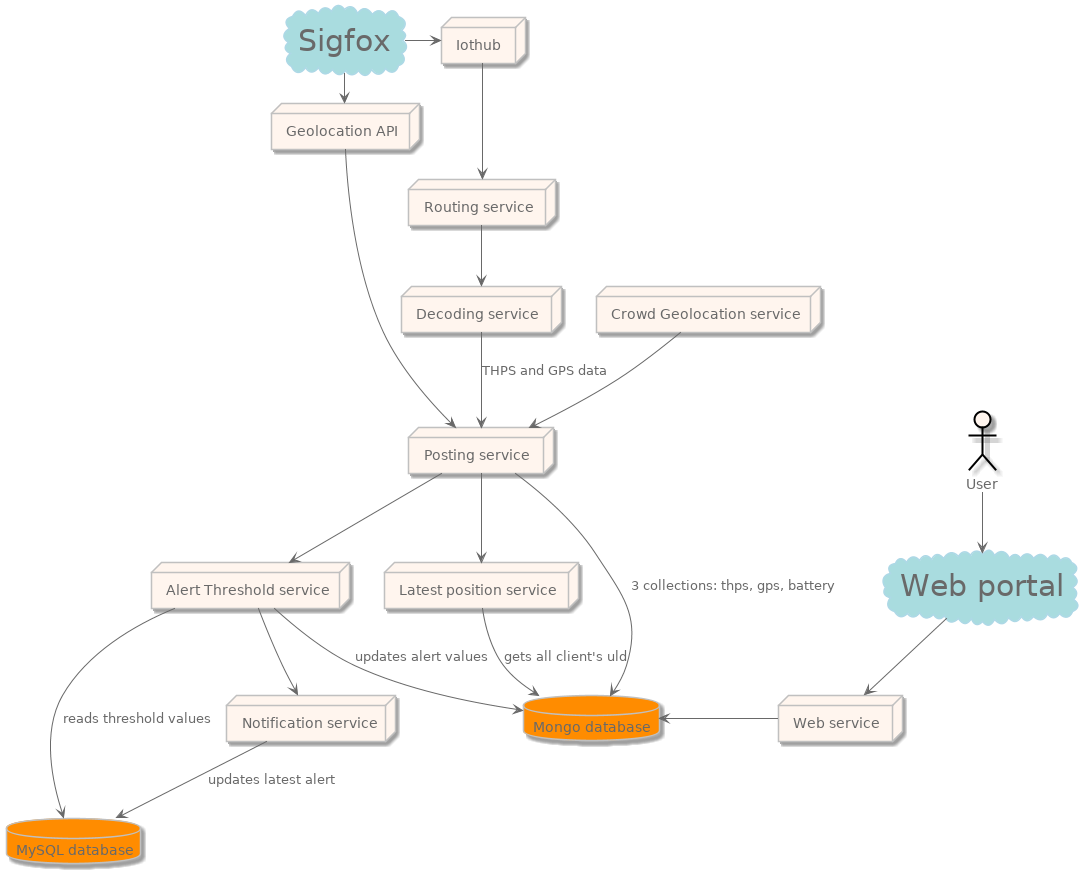
\includegraphics[scale=0.4]{servicesOverview}
            \caption{Plan de l'architecture}\label{fig:overview}
        \end{figure}

        \subsection{Services implémentés}
        \subsubsection{Decoding Service}
        C'est le premier service que j'ai eu à implémenter. 
        Les données des divers capteurs arrivent par ce service. Deux types de
        capteurs sont utilisés, l'un envoit des données de géolocalisation,
        l'autre envoit des données physique\footnote{température, pression,
        humidité, choc (shock): THPS.}. Il a alors la charge décoder un message
        binaire, puis d'en déterminer le type\footnote{GPS ou THPS}. ce service
        sert principalement à mettre en forme les données en \gls{json}, puis
        les envoyer à un autre micro-service. dans le cas où les données ne
        sont pas conformes, les données sont refusés, et le message est ignoré.
        Le principe de ce service est résumé par l'algorithme la figure
        \ref{fig:algo_decoding}.
        En sortie du micro-service, il ne faut pas trouver de données
        incohérentes, qui viendrait alors 
        polluer la base de données.

        \begin{figure}
            \centering
            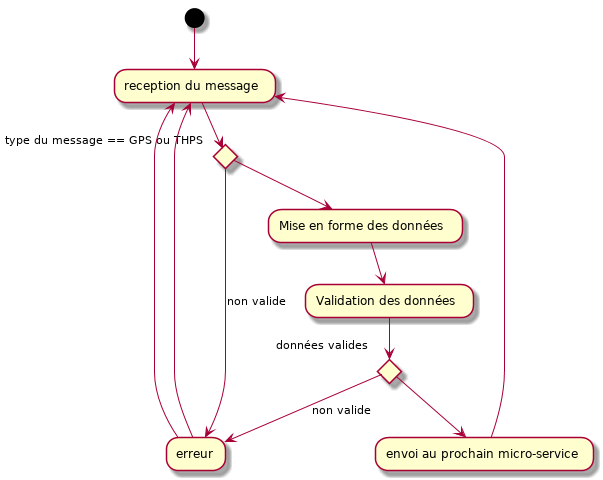
\includegraphics[scale=0.5]{algo_decoding}
            \caption{Fonctionnement du decoding}\label{fig:algo_decoding}
        \end{figure}

        \subsubsection{Posting service}
        Ce service est responsable de poster les données décodées et validées par le decoding service.
        En fonction du type de message, \textit{THPS} ou \textit{GPS}, les données vont être orienté vers un service différent,
        comme indiqué dans la figure \ref{fig:overview}. Ce service sert donc principalement d'aiguillage pour les messages.

        \subsubsection{Alert threshold service}
        Juste après le posting service, le message est traité par l'alert threshold service s'il est de type \textit{THPS}.
        Ce service à la responsabilité de confronter les valeurs contenues dans le message à des valeurs de références contenues dans
        une base de données. Si l'un des seuils est atteint, une alerte est transmise au \emph{notification service}.

        \subsection{Problèmes rencontrés}
        Le principal problème que j'ai rencontré sur ce projet, c'est que le code issu du prototype était extrêment pénible à lire, principalement 
        parce que son élaboration avait été négligée par son auteur. La plupart du temps a été passée à comprendre les lignes de
        code, et l'objectif de ce qui était codé à la base.

        \section{Mynabes}\label{subsec:mynabes}

        \begin{wrapfigure}{l}{0.30\textwidth}
            \centering
            
\includegraphics[width=0.30\textwidth]{mynabes}
        \end{wrapfigure}

        Mynabes est le projet d'une cliente au États-Unis.
        Cette derniere souhaitait créer une application 
        permettant de mettre en relation les voisins d'un
        même quartier.
        Ainsi l'enjeu était de pouvoir créer une application permettant~:
        \begin{itemize}
            \item De créer un post à la manière d'un réseau social, décrivant une demande, un service récompensé ou non
            \item À n'importe qui de pouvoir répondre à 
                cette demande et de contacter son auteur
        \end{itemize}

        Un utilisateur pouvait donc au sein de l'application accéder à une liste de poste, 
        mais aussi filter et rechercher dans cette liste de poste. En outre l'utilisateur
        a le choix d'accéder uniquement aux posts de son voisinage, ou alors son voisinage proche.
        Chaque post appartient à une catégorie, et pour chaque service rendu, un utilisateur peut être récompensé
        par l'auteur d'un post. La figure~\ref{fig:mynabes-usecase} résume les interactions générales sur l'application

        \begin{figure}
            \centering
            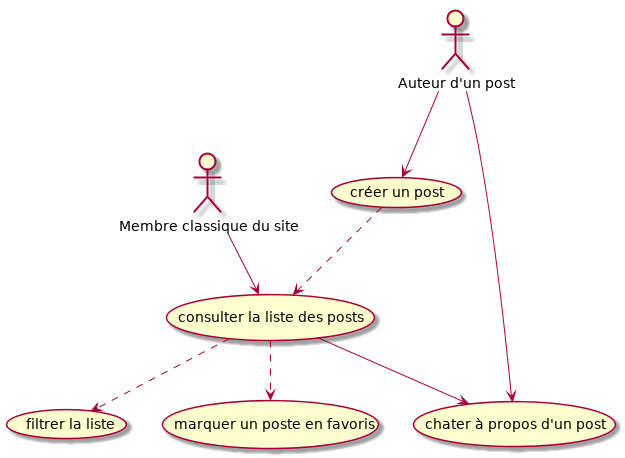
\includegraphics[scale=0.5]{mynabes-usecase}
            \caption{Cas d'utilisation de MyNabes}\label{fig:mynabes-usecase}
        \end{figure}

        \subsection{Architecture utilisée}
        Le projet a repris la même architecture que pour jobigo présenté à la
        page \pageref{subsec:jobigo}. On retrouve ainsi un projet côté serveur
        et l'application mobile en elle même. Le serveur est chargé de traiter
        les requêtes de l'application, et lui renvoyer les données demandées.
        L'application a elle la charge de mettre en forme les données et
        fournir une interface pour l'utilisateur afin qu'il puisse communiquer
        avec le serveur. L'\gls{api} est conçu en utilisant la convention \gls{rest}, 
        définie plus tôt dans le rapport (\emph{exemple: tableau \ref{table:rest}}).

        \subsection{Technologies utilisées}
        \begin{center}
            \begin{minipage}{0.20\textwidth}
                
\includegraphics[scale=0.1]{gitlab}
            \end{minipage}
            \begin{minipage}{0.20\textwidth}
                
\includegraphics[scale=0.1]{jenkins}
            \end{minipage}
            \begin{minipage}{0.20\textwidth}
                
\includegraphics[scale=0.2]{crashlytics}
            \end{minipage}
            \begin{minipage}{0.10\textwidth}
                
\includegraphics[scale=0.2]{laravel}
            \end{minipage}
        \end{center}

        Ce projet a été écrit en php avec Laravel\cite{laravel}, qui est un autre \gls{framework} destiné à construire des projets web. Personnellement
        je trouve que Laravel est plus simple d'utilisation que api-plateform. Ce dernier nécessite en effet beaucoup de configuration
        avant de pouvoir commencer à développer le projet, ce qui n'est pas le cas de Laravel.

        Ce projet partage des outils/technologies communs avec Jobigo, comme jenkins pour l'intégration continue, gitlab pour la gestion du code, et crashlytics pour la compilation et le déploiement continue de l'application.

        \subsection{Implémentation}

        \subsubsection{Actions de base}
        Au début du projet seulement une petite partie des fonctionnalités avait été développées.
        Ma première contribution à MyNabes a été de rajouter la possiblité dans l'\gls{api} d'accéder
        aux informations détaillée d'un post. 
        
        Par la suite j'ai également rajouté les fonctionnalité suivantes basiques~:~
        \begin{itemize}
            \item marquer un post en favoris
            \item signaler un post (pour contenu inapproprié par exemple)
            \item masquer un post
        \end{itemize}

        \subsubsection{La recherche de post}
        Une des actions de base que l'on peut retrouver dans ce genre d'application, c'est une fonction de recherche.
        Dans le cadre de mynabes, la fonction de recherche devait permettre à un utilisateur de rechercher un post grâce
        à une saisie de texte libre, puis pouvoir filter le résultat selon plusieurs critères, comme notamment la catégorie
        ou le type de récompense.

        Cette fonctionnalité se traduit par une requête SQL tenant compte de plusieurs paramètres, parfois invisible à l'utilisateur~:~
        \begin{itemize}
            \item Pour la recherche avec un texte libre, il fallait comparer le texte au titre du post, le nom de l'auteur, le contenu
            \item pour le filtrage il fallait tenir compte des différents attributs du post
            \item Il fallait aussi vérifier que le post faisait bien parti de son quartier
            \item Il fallait également écarter les posts volontairement masqués par l'utilisateur
            \item Il ne fallait pas non plus que le post apparaisse s'il avait été signalé
        \end{itemize}

        \subsubsection{Les notifications push}
        Ce projet d'application n'a pas fait exception à la règle, il a fallu établir des \glspl{push}.
        Cette fois çi il a été décidé de ne pas utiliser APNS pour les appareils sous iOS, mais d'utiliser 
        FCM pour s'occuper à la fois des appareil iOS et Android, ce qui a simplifié le travail. Il n'y avait donc
        qu'un seul de type à s'occuper, contrairement à jobigo. Le fonctionnement est toujours le même que pour la 
        figure~\ref{fig:notification}

        \subsection{Problèmes rencontrés}
        Pendant ce projet, le client a de temps en temps demandé des changements dans l'application. Il fallait donc en tenir
        compte, même si parfois il fallait radicalement changer un processus. En outre beaucoup de besoins étaient mal définis
        en amont par le client, il fallait donc soit le consulter, soit prendre des initiatives. Dans tous les cas cela pouvait ralentir le
        processus de développement.
        
\end{document}
